\documentclass[xcolor=pdftex,svgnames,table]{beamer}
\usepackage{latexsym,amssymb,amsmath,stmaryrd}
\usepackage[utf8]{inputenc}
\usepackage[T1]{fontenc}
\usepackage[francais]{babel}
\usepackage{pgf}
\usepackage{tikz}
\usetikzlibrary{arrows,patterns,plotmarks,shapes,snakes,er,3d,automata,%
backgrounds,topaths,trees,petri,mindmap}
\usepackage{pgfbaseimage}
\usepackage{ifpdf}
\ifpdf
\usepackage{graphicx}
\else
%\usepackage[dvips]{graphicx}
\usepackage{pstricks,pst-tree,pst-node}
\newpsobject{showgrid}{psgrid}{subgriddiv=1,griddots=10,gridlabels=6pt}
\fi
\usepackage{moreverb}
\usepackage[normalem]{ulem}
\usepackage{version}
\usepackage{url}
\usepackage{multicol}
\usepackage{listings}
\lstset{
  language=[ANSI]C, 
%  gobble=2, 
%  escapeinside="", 
  basicstyle=\ttfamily, 
%  directivestyle=\color{Fuchsia},
  identifierstyle = \color{DarkOrange},
  keywordstyle=\color{DarkGreen}, 
  commentstyle=\color{red}, 
%  numbers=left, 
%  numbersep=5pt, 
%  numberstyle=\scriptsize, 
%  moredelim=[is][\color{gray}\itshape]{/*}{*/}, 
%  moredelim=[is][\alert]{/+}{+/}, 
%  morecomment=[is]{/=}{=/}, 
%  morecomment=[in]{comment=}{,} 
%  fancyvrb=true 
} 

\newcommand{\binaire}[1]{\ensuremath{\underline{#1}}}
\newcommand{\C}[1]{\texttt{#1}}
\newcommand{\bbbn}{\ensuremath{\mathbb{N}}}
%%%%%%%%%%%%%%%%%%%%%%%%%%%%%%%%%%%%%%%%%%%%%%%%%%%%%%%%%%%%%%%%
%% ccBeamer 0.1, 2007-07-02                                   %%
%% Written by Sebastian Pipping <webmaster@hartwork.org>      %%
%% ---------------------------------------------------------- %%
%% Licensed under Creative Commons Attribution-ShareAlike 3.0 %%
%% http://creativecommons.org/licenses/by-sa/3.0/             %%
%%%%%%%%%%%%%%%%%%%%%%%%%%%%%%%%%%%%%%%%%%%%%%%%%%%%%%%%%%%%%%%%


%% Images
\newcommand{\CcImageBy}[1]{%
	
\includegraphics[scale=#1]{creative_commons/cc_by_30}%
}
\newcommand{\CcImageCc}[1]{%
	
\includegraphics[scale=#1]{creative_commons/cc_cc_30}%
}
\newcommand{\CcImageDevNations}[1]{%
	
\includegraphics[scale=#1]{creative_commons/cc_dev_nations_30}%
}
\newcommand{\CcImageNc}[1]{%
	
\includegraphics[scale=#1]{creative_commons/cc_nc_30}%
}
\newcommand{\CcImageNd}[1]{%
	
\includegraphics[scale=#1]{creative_commons/cc_nd_30}%
}
\newcommand{\CcImagePd}[1]{%
	
\includegraphics[scale=#1]{creative_commons/cc_pd_30}%
}
\newcommand{\CcImageSa}[1]{%
	
\includegraphics[scale=#1]{creative_commons/cc_sa_30}%
}
\newcommand{\CcImageSampling}[1]{%
	
\includegraphics[scale=#1]{creative_commons/cc_sampling_30}%
}
\newcommand{\CcImageSamplingPlus}[1]{%
	
\includegraphics[scale=#1]{creative_commons/cc_sampling_plus_30}%
}


%% Groups
\newcommand{\CcGroupBy}[1]{% zoom
	\CcImageBy{#1}%
}
\newcommand{\CcGroupByNc}[2]{% zoom, gap
	\CcImageBy{#1}\hspace*{#2}\CcImageNc{#1}%
}
\newcommand{\CcGroupByNcNd}[2]{% zoom, gap
	\CcImageBy{#1}\hspace*{#2}\CcImageNc{#1}\hspace*{#2}\CcImageNd{#1}%
}
\newcommand{\CcGroupByNcSa}[2]{% zoom, gap
	\CcImageBy{#1}\hspace*{#2}\CcImageNc{#1}\hspace*{#2}\CcImageSa{#1}%
}
\newcommand{\CcGroupByNd}[2]{% zoom, gap
	\CcImageBy{#1}\hspace*{#2}\CcImageNd{#1}%
}
\newcommand{\CcGroupBySa}[2]{% zoom, gap
	\CcImageBy{#1}\hspace*{#2}\CcImageSa{#1}%
}
\newcommand{\CcGroupDevNations}[1]{% zoom
	\CcImageDevNations{#1}%
}
\newcommand{\CcGroupNcSampling}[2]{% zoom, gap
	\CcImageNc{#1}\hspace*{#2}\CcImageSampling{#1}%
}
\newcommand{\CcGroupPd}[1]{% zoom
	\CcImagePd{#1}%
}
\newcommand{\CcGroupSampling}[1]{% zoom
	\CcImageSampling{#1}%
}
\newcommand{\CcGroupSamplingPlus}[1]{% zoom
	\CcImageSamplingPlus{#1}%
}


%% Text
\newcommand{\CcLongnameBy}{Attribution}
\newcommand{\CcLongnameByNc}{Attribution-NonCommercial}
\newcommand{\CcLongnameByNcNd}{Attribution-NoDerivs}
\newcommand{\CcLongnameByNcSa}{Attribution-NonCommercial-ShareAlike}
\newcommand{\CcLongnameByNd}{Attribution-NoDerivs}
\newcommand{\CcLongnameBySa}{Attribution-ShareAlike}

\newcommand{\CcNote}[1]{% longname
	This work is licensed under the \textit{Creative Commons #1 3.0 License}.%
}

\usetheme{classic}
\newcommand{\nowrite}{\put(10,-4){\includegraphics[scale=.05]{creative_commons/nopencil}}}
\newcommand{\youwrite}{\put(10,-4){
\includegraphics[scale=.05]{creative_commons/pencil}}}
\newcommand{\writethat}{
\includegraphics[scale=.05]{creative_commons/pencil}}
\newcommand{\aemporter}{\put(10,-6){
\includegraphics[scale=.05]{creative_commons/szymonraj_Shopping_bag}}}


%%% Titre -- cours 5
\title{Algorithmique et programmation.\\ Fonctions et procédures (2)}
\author{Pierre Boudes}
\date{\today}

%\includeonlyframes{current}

\begin{document}

%% Page de titre et licence CC.
\begin{frame}
        \titlepage
        \vfill
        \begin{center}
                \CcGroupByNcSa{0.83}{0.95ex}\\[2.5ex]
                {\tiny\CcNote{\CcLongnameByNcSa}}
                \vspace*{-2.5ex}
        \end{center}
\end{frame}

%%%%%%%%%%%%%%%%%%%%
\section[Plan]{}
\frame[label=plan]{\tableofcontents}
\section{Types char et double}
\subsection{Représentation des réels en virgule flottante}
\begin{frame}
    \frametitle{Représentation des réels en virgule flottante}
    \begin{itemize}
    \item La représentation informatique usuelle des réels s'inspire de la
      notation scientifique :
      \begin{align*}
        \pi &= 3,141592653589793\tag{pi}\\
        -700 \text{ milliards} &= -7 \times 10^{11}\tag{Paulson}\\
        h &= 6,626068 \times 10^{-34} \tag{Planck}\\
        \text{Univers} &= 1 \times 10^{80}  \tag{Atomes}
      \end{align*}\pause
\vspace{-.8cm}
\item Les bits sont séparés en :
  \begin{itemize}
  \item bit de signe\hfill (1 bit)
  \item mantisse \hfill (53 bits)
  \item exposant \hfill (11 bits)
  \end{itemize}\pause
\item En \textbf{double} précision (64 bits) :
  \begin{itemize}
\item exposant : entre $10^{-308}$ et $10^{308}$ (environ).
\item mantisse : 16 chiffres décimaux (environ).
  \end{itemize}\pause
\item Infini positif, infini négatif.
\item NaN : not a number.
    \end{itemize}
\end{frame}

\subsection[Types char, double et E/S]{Types et entrées sorties}
\begin{frame}
  \frametitle{Type double en C et entrées/sorties associées}
  
  \begin{itemize}
  \item Type des entiers relatifs  \alert{\C{int}}  (rappel) : 
    \begin{itemize}
    \item Déclaration et initialisation : \C{int n = -23;}.
    \item Représentation en complément à deux.
    \item E/S : \alert{\C{\%d}}.
    \end{itemize}
  \item Type des réels \alert{\C{double}} :
    \begin{itemize}
    \item Déclaration et initialisation : \C{double x = 3.14e-3;}.
    \item Représentation en virgule flottante sur 64 bits.
    \item E/S : \alert{\C{\%lg}} (mais plutôt \C{\%g} avec \C{printf}).
    \item \alert{Attention :} toujours mettre le point (équivalent
      anglais de la virgule) pour les constantes réelles (\C{1.0}).
    \end{itemize}
  \end{itemize}
\end{frame}

\begin{frame}
  \begin{block}{Entiers}
\C{int n;\\
...\\
printf("Entrer un nombre entier$\backslash$n");\\ 
scanf("\%d", \alert{\&}n);}
  \end{block}\pause

\begin{block}{Réels}
\C{double x;\\
...\\
printf("Entrer un nombre reel$\backslash$n");\\
scanf("\%lg", \alert{\&}x);\\ \pause
printf("Vous avez saisi : \%g$\backslash$n", x);
}
\end{block}
 Remarque : on tombe vite sur un problème (boucle infinie) avec scanf car cette fonction
 s'occupe à la fois de reconnaître ce que tape l'utilisateur et
 de \emph{purger} cette entrée. Mais scanf ne purge pas ce qui n'est
 pas reconnu (démo) ! Il faudra séparer purge et reconnaissance.
\end{frame}



\begin{frame}
  \frametitle{Type char  en C et entrées/sorties associées}  
Type des caractères \alert{\C{char}} :
    \begin{itemize}
    \item Déclaration et initialisation : \C{char c = 'A';}.
    \item Représentation sur 8 bits, ASCII, ISO-8859-x, UTF-8.
    \item E/S : \alert{\C{\%c}}.
    \end{itemize}

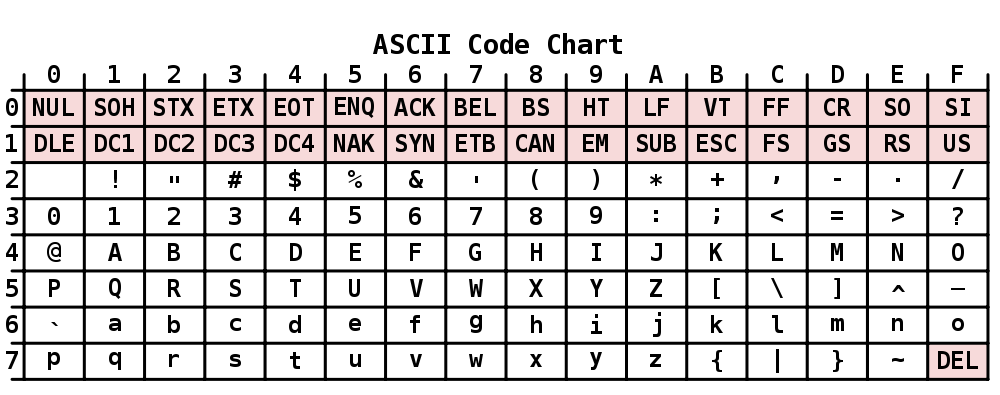
\includegraphics[scale=0.31]{img/1000px-ASCII_Code_Chart.png}

\vspace{-0.3cm}
{\scriptsize\hfill  Source: Wikimedia Commons, public domain.}
\end{frame}


\begin{frame}
  
  \begin{block}{Caractères}
\C{char c;\\
...\\
printf("Entrer un caractère$\backslash$n");\\
scanf("\%c", \alert{\&}c);
}
\\ \pause
    \alert{Attention :} mieux vaut utiliser 
    \C{scanf("\textvisiblespace\%c", \alert{\&}c);}
  \end{block}\pause

\begin{block}{Chaînes de caractères (semaine prochaine) \aemporter}
\C{char nom[64];\\
...\\
printf("Entrer votre nom$\backslash$n");\\
scanf("\%s", nom);\\ \pause
}
\end{block}

\end{frame}

\subsection[Conversions automatiques]{Conversions automatiques entre types}
\begin{frame}[fragile]
  \frametitle{Conversions  automatiques entre types}

  \begin{itemize}
\item Sans changement de représentation  :
  \begin{itemize}
    \item \C{char} vers \C{int}
    \item \C{int} vers \C{char} (troncature)
  \end{itemize}\pause
  \begin{lstlisting}[basicstyle=\ttfamily\small] 
  char c;
  int n;
  
  n = 'A' + 1; /* voir table ascii */
  c = n + 24; /* quel caractere vaut c ? */
   \end{lstlisting}  
 \item Avec changement de représentation :
    \begin{itemize}
    \item char ou entiers vers réels
    \item réels vers entiers ou char
    \end{itemize}
  \begin{lstlisting}[basicstyle=\ttfamily\small] 
  double x;
  int n;
  
  n = 3.1; /* que vaut n ? */
  x = n; 
   \end{lstlisting} 
  \end{itemize}
\end{frame}

\section{Fonctions et procédures, compléments}

\subsection{Rappel sur les fonctions en C}

\begin{frame}
  \frametitle{Rappel sur les fonctions en C\nowrite}
 Utilisation des fonctions :
  \begin{itemize}
    \item \structure{déclaration} \textbf{types} (\C{int}, \C{char},
      \C{double}, \C{void}) des paramètres et de la valeur de retour;
    \item \structure{définition}  code, paramètres formels (chacun est
      une variable locale);
    \item \structure{appel} paramètres effectifs (chaque expression
      donnant sa valeur au paramètre formel correspondant), \textbf{espace mémoire}.
  \end{itemize}
\pause 
\pause
Nous allons voir de façon plus précise cette question
d'espace mémoire, avec la pile d'appel.

\pause avant cela, quelques compléments (\C{void}, bibliothèques de fonction).
\end{frame}


\subsection[Procédures]{Fonctions sans valeurs de retour (void)}
\begin{frame}[fragile]
  \frametitle{Fonctions sans valeurs de retour (void)}

On parle plutôt de procédure ou de routine car l'analogie avec les
fonctions mathématiques est perdue.

 \begin{block}{Déclarer}
    \begin{lstlisting}[basicstyle=\ttfamily\small] 
void afficher_valeurs(int x, int y);
     \end{lstlisting}
  \end{block}

  \begin{block}{Appeler}
  \begin{lstlisting}[basicstyle=\ttfamily\small] 
afficher_valeurs(5, 3);
   \end{lstlisting}  
  \end{block}

  \begin{block}{Définir}
Comme d'habitude mais pas de \C{return} (ou \C{return sans argument}).
\end{block}
\end{frame}

%\subsection[Procédures]{Fonctions sans valeurs de retour (void)}
\begin{frame}[fragile]
  \frametitle{Fonctions sans arguments}

 \begin{block}{Déclarer}
    \begin{lstlisting}[basicstyle=\ttfamily\small] 
int nombre_aleatoire();
int saisie_utilisateur();
     \end{lstlisting}
  \end{block}

  \begin{block}{Appeler}
  \begin{lstlisting}[basicstyle=\ttfamily\small] 
  int n;
  int secret;

  secret = nombre_aleatoire();

  n = saisie_utilisateur();
   \end{lstlisting}  
  \end{block}

  \begin{block}{Définir}
Comme d'habitude.
\end{block}
\end{frame}

\subsection[math.h]{Utiliser les fonctions d'une bibliothèque}

\begin{frame}[fragile]
  \frametitle{Utiliser les fonctions d'une bibliothèque (math.h)}
Utilisation de la bibliothèque math.h 
\begin{verbatim}
$ man math
\end{verbatim}
  \begin{block}{Déclarer}
    \begin{lstlisting}[basicstyle=\ttfamily\small] 
#include <math.h>
     \end{lstlisting}
  \end{block}

  \begin{block}{Appeler}
  \begin{lstlisting}[basicstyle=\ttfamily\small] 
  double x;

  x = log(3.5);
    \end{lstlisting}  
  \end{block}

  \begin{block}{Définir}
\begin{verbatim}
$ gcc -lm -Wall prog.c -o prog.exe
\end{verbatim}
 \end{block}
\end{frame}


\section{Traces et pile d'appel}
\subsection{Traces : flot de contrôle et données}
\begin{frame}
  \frametitle{Traces (rappel)}

Pour  étudier l'exécution de nos programmes, nous faisons la trace de chaque appel de
chaque fonction que l'on a défini (les fonctions utilisateur, pas les fonctions externes, comme printf).

{
\rowcolors{2}{LightSkyBlue}{LightSteelBlue} %\arrayrulecolor{green!75!gray}
\small
      \setlength{\unitlength}{\tabcolsep}
          \begin{tabular}[t]{|c|c|l|}
          \multicolumn{3}{l}{\C{main()}}\\ \hline
          ligne & n & Affichage \\ \hline
          initialisation  & 9 & \\ \hline
          16 & & \\ \hline
          \rowcolor{LightYellow}
          & & \multicolumn{1}{>{\columncolor{LightYellow}}r|}{
            \put(1,0){\noindent
              \begin{tabular}[t]{|c|c|c|l|}
          \multicolumn{4}{l}{\C{est\_premier(9)}}\\ \hline
          ligne & n & i & Affichage \\  \hline
          initialisation  & 9 & ? & \\ \hline
         34 &  & 2 & \\ \hline
         40  &  & 3 & \\ \hline
         38  &\multicolumn{3}{|>{\columncolor{MediumSpringGreen}}l|}{renvoie FALSE}\\ \hline 
        \end{tabular}
              }
          }\\ \hline 
          22 & & 9 n'est pas premier\\ \hline
          26 &\multicolumn{2}{|>{\columncolor{LightSteelBlue}}l|}{renvoie EXIT\_SUCCESS}\\ \hline
          \end{tabular}
}
\end{frame}


\begin{frame}[fragile,label=current1]
  \frametitle{Focus sur le passage de valeurs}
  Notez que les fonctions communiquent \textbf{des valeurs}, pas des noms de
  variables.
\begin{columns}
\scriptsize
  \begin{column}[t]{3.7cm}
 \begin{lstlisting}[numbers=left,basicstyle=\ttfamily\scriptsize]
void permute_valeurs(int a,int b);

int main() {
    int x = 1;
    int y = 2;    
    permute_valeurs(x,y);
    printf("x = %d et y = %d\n",x,y);
    return EXIT_SUCCESS;
}

void permute_valeurs(int a,int b) {
    int aux;
    aux = a;
    a = b;
    b = aux;
}\end{lstlisting}
\vspace{.4cm}
 \end{column}
\begin{column}[t]{4cm}
\pause
\rowcolors{2}{LightSkyBlue}{LightSteelBlue} %\arrayrulecolor{green!75!gray}
        \setlength{\unitlength}{\tabcolsep}
      \hspace{-5.5cm} \begin{tabular}[t]{|r|c|c|l|}
          \multicolumn{4}{l}{\C{main()}}\\ \hline
          ligne & x & y & Affichage \\ \hline
          initialisation  & 1 & 2 & \\ \hline
          6 &   & &\pause \\ \hline
          \multicolumn{4}{|r|}{
            \put(1,4){\noindent
              \begin{tabular}[t]{|r|c|c|c|l|}
                \multicolumn{5}{|l}{\C{permute\_valeurs(1, 2)}}\\ \hline
                ligne & a & b & aux & Aff. \\ \hline
                initialisation  & 1 & 2 & ? &\pause \\ \hline
                13 &  &  & 1 & \\ \hline
                14 & 2 &  &  & \\ \hline
                15 &  &  1  &  & \\ \hline
                16 &\multicolumn{4}{|>{\columncolor{MediumSpringGreen}}l|}{ne renvoie rien}\\ \hline
              \end{tabular}
            }} \\ \hline
          7  &  &  & \C{x = \pause1 et y = 2} \\ \hline
          8 &\multicolumn{3}{|l|}{SORTIE AVEC SUCCÈS}\\ \hline
        \end{tabular}
  \end{column}
\end{columns}
\end{frame}
\begin{frame}[fragile,label=current]
  \frametitle{Un exemple avec plus d'appels de fonctions}
\vspace{-0.5cm}
\begin{columns}
\scriptsize
  \begin{column}[t]{3.7cm}
 \begin{lstlisting}[numbers=left,basicstyle=\ttfamily\scriptsize]
double maximum(double x, double y);
double valeur_absolue(double x);
int main() {
    double a = -4.2;c
    double b = 1.3; 
    a = valeur_absolue(a) + valeur_absolue(b);
    printf("%g\n", a);
    return EXIT_SUCCESS;
}
double maximum(double x, double y) {
    if (x > y) {
        return x;
    }
    return y;
}
double valeur_absolue(double x) {
    return maximum(x, -x);
}
\end{lstlisting}
\vspace{0.5cm}
 \end{column}
\begin{column}[t]{4cm}
\pause~
\only<-6>{%
\rowcolors{2}{LightSkyBlue}{LightSteelBlue}
% \arrayrulecolor{green!75!gray}
        \setlength{\unitlength}{\tabcolsep}
      \hspace{-5cm} \begin{tabular}[t]{|r|c|c|l|}
          \multicolumn{4}{l}{\C{main()}}\\ \hline
          ligne & a & b & Aff. \\ \hline
          initialisation  & -4.2 & 1.3 & \\ \hline
          6\pause & & &  \multicolumn{1}{ >{\columncolor{LightSteelBlue}}r|
          }{\put(2,0){\C{valeur\_absolue(-4.2)}}} \\ \hline
          \multicolumn{4}{|r|}{\only<7>{\cellcolor{LightGreen}}
            \put(1,1){\noindent
              \begin{tabular}[t]{|r|c|}\hline
                ligne  & x    \\ \hline
                init.  & -4.2 \\ \hline
                17 \pause & \multicolumn{1}{ >{\columncolor{LightSteelBlue}}r|
                }{\put(2,0){\C{maximum(-4.2, 4.2)}}}\\ \hline
                \multicolumn{2}{r|}{\only<7>{\cellcolor{LightGoldenrod}}
                  \put(1,1){\noindent
                    \begin{tabular}[t]{|r|c|c|}\hline
                      ligne & x & y \\ \hline
                      init.  & -4.2 & 4.2 \\ \hline
                      14\pause &\multicolumn{2}{|>{\columncolor{MediumSpringGreen}}l|}{renvoie 4.2}\\ \hline
                    \end{tabular}
                  }} \\ \hline
                17 \pause &\multicolumn{1}{|>{\columncolor{MediumSpringGreen}}l|}{renvoie 4.2}\\ \hline
              \end{tabular}
            }} \\ \hline
          \rowcolor{LightSkyBlue} 6 & & &\multicolumn{1}{ >{\columncolor{LightSkyBlue}}r| }{\put(2,0){\C{valeur\_absolue(1.3)}}}\\ \hline
          \multicolumn{4}{|r|}{\only<7>{\cellcolor{LightGreen}}
            \put(1,1){\noindent
              \begin{tabular}[t]{|r|c|}\hline
                ligne  & x    \\ \hline
                init.  & 1.3 \\ \hline
                17 & \multicolumn{1}{ >{\columncolor{LightSteelBlue}}r|
                }{\put(2,0){\C{maximum(1.3, -1.3)}}}\\ \hline
                \multicolumn{2}{|r|}{\only<7>{\cellcolor{LightGoldenrod}}
                  \put(1,1){\noindent
                    \begin{tabular}[t]{|r|c|c|}\hline
                      ligne & x & y \\ \hline
                      init.  & 1.3 & -1.3 \\ \hline
                      12 &\multicolumn{2}{|>{\columncolor{MediumSpringGreen}}l|}{renvoie 1.3}\\ \hline
                    \end{tabular}
                  }} \\ \hline
                17 &\multicolumn{1}{|>{\columncolor{MediumSpringGreen}}l|}{renvoie 1.3}\\ \hline
              \end{tabular}
            }} \\ \hline
          6  & 5.5 &  &  \\ \hline
          7  &  &  & \C{5.5} \\ \hline
          8 &\multicolumn{3}{|l|}{SUCCÈS}\\ \hline
        \end{tabular}
}%fin only
\only<7->{%
\rowcolors{2}{LightGreen}{LightGreen}
% \arrayrulecolor{green!75!gray}
        \setlength{\unitlength}{\tabcolsep}
      \hspace{-5cm} \begin{tabular}[t]{|r|c|c|l|}
          \multicolumn{4}{l}{\C{main()}}\\ \hline
          ligne & a & b & Aff. \\ \hline
          initialisation  & -4.2 & 1.3 & \\ \hline
          6\pause & & &  \multicolumn{1}{ >{\columncolor{LightSteelBlue}}r|
          }{\put(2,0){\C{valeur\_absolue(-4.2)}}} \\ \hline
          \multicolumn{4}{|r|}{\only<7>{\cellcolor{LightGreen}}
            \put(1,1){\noindent
\rowcolors{2}{LightGoldenrod}{LightGoldenrod}
              \begin{tabular}[t]{|r|c|}\hline
                ligne  & x    \\ \hline
                init.  & -4.2 \\ \hline
                17 \pause & \multicolumn{1}{ >{\columncolor{LightSteelBlue}}r|
                }{\put(2,0){\C{maximum(-4.2, 4.2)}}}\\ \hline
                \multicolumn{2}{r|}{\only<7>{\cellcolor{LightGoldenrod}}
                  \put(1,1){\noindent
\rowcolors{2}{LightSkyBlue}{LightSkyBlue}
                    \begin{tabular}[t]{|r|c|c|}\hline
                      ligne & x & y \\ \hline
                      init.  & -4.2 & 4.2 \\ \hline
                      14\pause &\multicolumn{2}{|>{\columncolor{MediumSpringGreen}}l|}{renvoie 4.2}\\ \hline
                    \end{tabular}
                  }} \\ \hline
                17 \pause &\multicolumn{1}{|>{\columncolor{MediumSpringGreen}}l|}{renvoie 4.2}\\ \hline
              \end{tabular}
            }} \\ \hline
          \rowcolor{LightSkyBlue} 6 & & &\multicolumn{1}{ >{\columncolor{LightSkyBlue}}r| }{\put(2,0){\C{valeur\_absolue(1.3)}}}\\ \hline
          \multicolumn{4}{|r|}{\only<7>{\cellcolor{LightGreen}}
            \put(1,1){\noindent
\rowcolors{2}{LightGoldenrod}{LightGoldenrod}
              \begin{tabular}[t]{|r|c|}\hline
                ligne  & x    \\ \hline
                init.  & 1.3 \\ \hline
                17 & \multicolumn{1}{ >{\columncolor{LightSteelBlue}}r|
                }{\put(2,0){\C{maximum(1.3, -1.3)}}}\\ \hline
                \multicolumn{2}{|r|}{\only<7>{\cellcolor{LightGoldenrod}}
                  \put(1,1){\noindent
\rowcolors{2}{LightSkyBlue}{LightSkyBlue}
                    \begin{tabular}[t]{|r|c|c|}\hline
                      ligne & x & y \\ \hline
                      init.  & 1.3 & -1.3 \\ \hline
                      12 &\multicolumn{2}{|>{\columncolor{MediumSpringGreen}}l|}{renvoie 1.3}\\ \hline
                    \end{tabular}
                  }} \\ \hline
                17 &\multicolumn{1}{|>{\columncolor{MediumSpringGreen}}l|}{renvoie 1.3}\\ \hline
              \end{tabular}
            }} \\ \hline
          6  & 5.5 &  &  \\ \hline
          7  &  &  & \C{5.5} \\ \hline
          8 &\multicolumn{3}{|l|}{SUCCÈS}\\ \hline
        \end{tabular}
}%fin only
  \end{column}
\end{columns}
\end{frame}
\subsection{Traces : la mémoire et le temps}
\begin{frame}
  \frametitle{Traces : la mémoire  et le temps}
La trace d'un programme donne schématiquement ce type de dessin :
\begin{columns}
\column[T]{6.5cm}
\begin{itemize}
  \item<3-> verticalement, c'est le temps
  \item<3-> et horizontalement, l'occupation mémoire
  \item<4-> un appel de fonction occupe une portion de mémoire, puis la
    libère. 
\item<5-> la trace représente réellement ce qui arrive dans vos
  programmes (durée de vie et localisation en mémoire des variables, etc.).
\end{itemize}
 \uncover<6->{
\structure{Un appel de fonction peut-il modifier la mémoire d'une
  fonction appelante ?}}
\column[T]{4.5cm}
\small
\vspace{-0.5cm}
\only<2->{\hspace{-0.7cm}\noindent\begin{tikzpicture}
\tikzstyle{every node}=[anchor=base]
\only<3->{\tikzset{axis/.style={fill=none}}}
\only<2>{\tikzset{axis/.style={color=white,fill=white,draw=white}}}
% Axis
  \draw[axis,arrows = ->] (-.7,5.9) -- (4.2,5.9);
  \draw(4.1,6) node[axis,anchor=base east] {mémoire};
  \draw[axis,arrows = ->] (-.6,6.1) -- (-.6,-.5);
  \draw(-.8,-.2) node[axis,rotate=-90,anchor=base east] {temps};
%
 \draw (0, 5.6) node {main()};
  \filldraw[fill=LightGreen,draw=Green] (-0.5,-0.25) rectangle
  (1,5.5); 
  \draw[pattern color=Green, pattern=north east lines,draw=none] (-0.5,-0.25) rectangle
  (0,5.5); 
 \draw (0.25, 5.25) node {\C{x}};
  \draw[draw=Green] (0.5,-0.25) -- (0.5,5.5);
  \draw (0.75, 5.25) node {\C{y}};
%
 \draw (1.75, 5.1) node {max(1,2)};
  \filldraw[fill=LightGoldenrod, draw=DarkGoldenrod] (1,4) rectangle (2.5,5); 
  \draw[pattern color=DarkGoldenrod, pattern=north east lines,draw=none] (1,4) rectangle
  (1.5,5); 
  \draw (2.25, 4.75) node {\C{b}};
  \draw[draw=DarkGoldenrod] (2,4) -- (2,5); 
  \draw (1.75, 4.75) node {\C{a}};
%
  \draw (1.75, 3.6) node {\C{f(8)}};
  \filldraw[fill=PowderBlue,draw=RoyalBlue]
  (1,0) rectangle (2.5,3.5); 
  \draw[pattern color=RoyalBlue, pattern=north east lines,draw=none]
  (1,0) rectangle  (1.5,3.5); 
  \draw (1.75, 3.25) node {\C{z}};
  \draw[draw=RoyalBlue] (2,0) -- (2,3.5); 
  \draw (2.25, 3.25) node {\C{r}};
%
  \draw (3, 3.1) node {\C{g(2)}};
  \filldraw[fill=Salmon,draw=Crimson] (2.5,2) rectangle(3.5,3); 
  \draw[pattern color=Crimson, pattern=north east lines,draw=none]
  (2.5,2) rectangle  (3,3);
  \draw (3.25, 2.75) node {\C{n}};
%
  \filldraw[fill=LightGoldenrod, draw=DarkGoldenrod] (2.5,.5) rectangle
  (4,1.5); 
  \draw[pattern color=DarkGoldenrod, pattern=north east lines,draw=none] (2.5,.5) rectangle
  (3,1.5); 
  \draw (3.25, 1.6) node {max(2,-1)};
  \draw (3.25, 1.25) node {\C{a}};
  \draw[draw=DarkGoldenrod] (3.5,.5) -- (3.5,1.5);
  \draw (3.75, 1.25) node {\C{b}};
\end{tikzpicture}}
  \end{columns}
\end{frame}

\subsection{Pile d'appel}
\begin{frame}
  \frametitle{Pile d'appel}
\begin{columns}
\column[T]{4cm}
On parle de \alert{pile d'appel} car les appels de fonctions
s'empilent... \emph{comme sur une pile
    d'assiettes.}

\uncover<13->{
\structure{Peut-on avoir deux assiettes identiques dans la pile ? (La même
  fonction avec des contenus différents)}}

% de contenus différents
\column[T]{7.5cm}
\small
\noindent\begin{tikzpicture}[rotate=90]
\tikzstyle{every node}=[anchor=base]
\tikzset{axis/.style={fill=none}}
\tikzset{fonction/.style={rotate=90}}
% Axis
  \draw[axis,arrows = ->] (-.7,5.9) -- (4.2,5.9);
  \draw(4.1,6) node[axis,rotate=90,anchor=base east] {mémoire};
  \draw[axis,arrows = ->] (-.6,6.1) -- (-.6,-.5);
  \draw(-.8,-.2) node[axis,anchor=base east] {temps};
%
\uncover<1,3->{
  \draw (0, 5.6) node[fonction] {main()};
  \filldraw[fill=LightGreen,draw=Green] (-0.5,-0.25) rectangle
  (1,5.5); 
  \draw[pattern color=Green, pattern=north east lines,draw=none] (-0.5,-0.25) rectangle
  (0,5.5); 
 \draw (0.25, 5.25) node {\C{x}};
  \draw[draw=Green] (0.5,-0.25) -- (0.5,5.5);
  \draw (0.75, 5.25) node {\C{y}};
}
%
\uncover<1,4,12->{
 \draw (1.75, 5.1) node[fonction] {max(1,2)};
  \filldraw[fill=LightGoldenrod, draw=DarkGoldenrod] (1,4) rectangle (2.5,5); 
  \draw[pattern color=DarkGoldenrod, pattern=north east lines,draw=none] (1,4) rectangle
  (1.5,5); 
  \draw (2.25, 4.75) node {\C{b}};
  \draw[draw=DarkGoldenrod] (2,4) -- (2,5); 
  \draw (1.75, 4.75) node {\C{a}};
}
%
\uncover<1,6-10,12->{
  \draw (1.75, 3.6) node[fonction] {\C{f(8)}};
  \filldraw[fill=PowderBlue,draw=RoyalBlue]
  (1,0) rectangle (2.5,3.5); 
  \draw[pattern color=RoyalBlue, pattern=north east lines,draw=none]
  (1,0) rectangle  (1.5,3.5); 
  \draw (1.75, 3.25) node {\C{z}};
  \draw[draw=RoyalBlue] (2,0) -- (2,3.5); 
  \draw (2.25, 3.25) node {\C{r}};
}
%
\uncover<1,7,12->{
  \draw (3, 3.1) node[fonction] {\C{g(2)}};
  \filldraw[fill=Salmon,draw=Crimson] (2.5,2) rectangle(3.5,3); 
  \draw[pattern color=Crimson, pattern=north east lines,draw=none]
  (2.5,2) rectangle  (3,3);
  \draw (3.25, 2.75) node {\C{n}};
}
%
\uncover<1,9,12->{
  \filldraw[fill=LightGoldenrod, draw=DarkGoldenrod] (2.5,.5) rectangle
  (4,1.5); 
  \draw[pattern color=DarkGoldenrod, pattern=north east lines,draw=none] (2.5,.5) rectangle
  (3,1.5); 
  \draw (3.25, 1.6) node[fonction] {max(2,-1)};
  \draw (3.25, 1.25) node {\C{a}};
  \draw[draw=DarkGoldenrod] (3.5,.5) -- (3.5,1.5);
  \draw (3.75, 1.25) node {\C{b}};
}
\end{tikzpicture}
\end{columns}
\end{frame}

\begin{frame}[fragile]
  \frametitle{Factorielle récursive (teaser)}
  \begin{block}{Définition}
    Une fonction récursive est une fonction dont la définition fait
    appel à la fonction \emph{elle-même}.
  \end{block}

\pause
Il y a une forte analogie avec les maths : $(n + 1)! = (n + 1) \times n!$

\pause
\begin{lstlisting}[escapechar={\%},basicstyle=\ttfamily\small] 
int factorielle(int n)
{
    if (n < 2) /* cas de base */
    {
         return 1;
    } 
    return n * factorielle(n - 1); 
}
\end{lstlisting}
\end{frame}

\section[Démos]{Longue démo (menu)}
\begin{frame}
  \frametitle{Longue démo (menu)}
\end{frame}
\end{document}

% revenir sur :
%-l'appel au cours suivant : paramètre et expression, pile d'appel.
%-la grammaire des identificateurs